\documentclass{llncs}

\usepackage{listings}
\usepackage{url}
\usepackage{graphicx} %png
\usepackage{subfigure} %placing pictures side-by-side
\usepackage{pifont}	%ding
\usepackage[usenames,dvipsnames]{color}	%text color
\usepackage{amssymb, amsmath}
\usepackage{ifthen}
\usepackage{marginnote}

%define JavaScript listing:
\definecolor{lightgray}{rgb}{.9,.9,.9}
\definecolor{darkgray}{rgb}{.4,.4,.4}
\definecolor{purple}{rgb}{0.65, 0.12, 0.82}

\lstdefinelanguage{JavaScript}{
  keywords={typeof, new, true, false, catch, function, return, null, catch, switch, var, if, in, while, do, else, case, break},
  keywordstyle=\color{blue}\bfseries,
  ndkeywords={class, export, boolean, throw, implements, import, this},
  ndkeywordstyle=\color{darkgray}\bfseries,
  identifierstyle=\color{black},
  sensitive=false,
  comment=[l]{//},
  morecomment=[s]{/*}{*/},
  commentstyle=\color{purple}\ttfamily,
  stringstyle=\color{red}\ttfamily,
  morestring=[b]',
  morestring=[b]"
}
\lstset{
   language=JavaScript,
   backgroundcolor=\color{lightgray},
   extendedchars=true,
   basicstyle=\footnotesize\ttfamily,
   showstringspaces=false,
   showspaces=false,
   numbers=left,
   numberstyle=\footnotesize,
   numbersep=9pt,
   tabsize=2,
   breaklines=true,
   showtabs=false,
   captionpos=b
}

% cirnum command to print numbers in circles within text
\newcounter{dingdistance}
\setcounter{dingdistance}{191}
\newcommand{\circnum}[1]{%
  \addtocounter{dingdistance}{#1}%
  \ding{\value{dingdistance}}%
  \setcounter{dingdistance}{191}}

% \todo command
\newcommand{\todo}[1][EMPTY]{%
\null\marginnote[$\rightarrow$]{$\leftarrow$}%
\ifthenelse{\equal{#1}{EMPTY}}%
{[\textsc{TODO}]}%
{[\textsc{TODO:} #1]}%
}
% \needcite command
\newcommand{\needcite}[1][EMPTY]{%
\null\marginnote[$\rightarrow$]{$\leftarrow$}%
\ifthenelse{\equal{#1}{EMPTY}}%
{[\textsc{citation needed}]}%
{[\textsc{citation needed from} #1]}%
}

% packed lists
\newenvironment{packed_enumerate}{
\begin{enumerate}
  \setlength{\itemsep}{1pt}
  \setlength{\parskip}{0pt}
  \setlength{\parsep}{0pt}
}{\end{enumerate}}
\newenvironment{packed_itemize}{
\begin{itemize}
  \setlength{\itemsep}{1pt}
  \setlength{\parskip}{0pt}
  \setlength{\parsep}{0pt}
}{\end{itemize}}
\newenvironment{packed_description}{
\begin{description}
  \setlength{\itemsep}{2pt}
  \setlength{\parskip}{0pt}
  \setlength{\parsep}{0pt}
}{\end{description}}

\begin{document}
\frontmatter
\pagestyle{headings}

\title{Cloud9 - gitc extension}
\author{Markus Kahl \and Stephanie Platz \and Patrick Schilf \\~ \small{advisors: Jens Lincke \and Prof. Dr. Robert Hirschfeld} }
\subtitle{Seminar Web-based Software Development Environments}
\institute{Hasso Plattner Institut \\ University of Potsdam, Germany}
\date{2011-02-18}

\maketitle

\begin{abstract}
\label{abstract} % markus
A very nice abstract.
\end{abstract}

\section{Introducing Web-based Software Development}
\label{sec:Introduction}

\begin{itemize}
	\item why do we want to do web-dev?
	\item mention Bret Victor talk http://vimeo.com/36579366 ?
	\item pros and cons in generall
\end{itemize}

\subsection{Environments}
\begin{itemize}
	\item list some environments, especially c9 ;)
	\item Jens list (dart, lively, ...)
	\item brackets
	\item collide
\end{itemize} %patrick
\section{Cloud9 by Example}
\label{sec:Motivation}

%\begin{itemize}
%	what c9 can do
%	Tetris
%	how was our development process (team of 3 (2 know git already), cloud9 dashboard, setting up c9 %project (github or bitbucket or without any of them))
%	where do we had problems,
%	our pros and cons for cloud9
%\end{itemize}

%more detailed description of git console
%include Cloud9 Screenshot
%include Tetris Screenshot
After registering for an account on the Cloud9 website or logging in through GitHub or BitBucket,
the user is led to the Dashboard where he can create new or maintain existing projects as well as access those
shared with him by other members.
Cloud9 supports many languages which amongst others are NodeJS, Javascript, HTML, CSS, Python, Ruby, PHP, C/C++, C\#, Java, and Scala.
While the first two of the mentioned are fully supported in terms of running and debugging other languages are only provided with syntax highlighting.
Once a workspace is created - either from scratch or by cloning from a URL from GitHub or BitBucket -
and the project is launched, the actual editing environment appears.
The user interface is arranged into three parts. The top is covered by a menu bar, followed by a navigation pane
on the left side of the screen and the editing window on the right.
At the bottom of the screen is an expandable git command shell, which accepts the entire range of Git commands.
The menu includes the mandatory items known from any desktop application such as file or edit operations, text search or view settings.
The navigation pane involves various views, accessible through tab icons. The most important one is the project explorer,
which displays all project files in a tree view. Here project files and folders can be edited, deleted or newly created.
Files that cannot be created or edited in Cloud9, such as images, can be dragged and dropped straight from a local hard disk.
Other views include Run \& Debug operations, Server Deployment or text editor settings.
The latter serves the actual coding purposes and supports multiple tabs. Under the hood runs an instance of the Ace
Editor\footnote{\url{http://ace.ajax.org/}}, originally known as Bespin and initially developed by Mozilla Labs,
and provides the user with many of the mandatory text editing features such as syntax highlighting, grouped code indention, and line numbers.
The new release also allows code completion, which has previously only been supported for some commands and
function or variable names that already appeared in one document.
A more detailed view on the Ace editor, its backend components and functionality is provided in Chapter ~\needcite. 

\subsection{Developing Tetris}
There is not much to say about Tetris, one of the world's most famous computer games. Single objects composed out of four
squares, that fall from the top border of the rectangular playing field, need to be arranged to form complete,
horizontal lines at the bottom of the field.
Our Javascript based implementation offers two players to battle each other with the use of a key shared keyboard.
Players score by dropping objects and generating unbroken lines. Accomplishing more than one line at once will
add the corresponding number of lines to the opponent player's field.
The first player running out of space for new spawning objects loses.
We duplicated the shapes of the original game and included six different levels.
Each level upgrade results in a higher score for each dropped object and cleared line as well as in a higher falling speed of the objects.

%include workflow illustration
Apart from designing the elements of the graphical user interface, which required the use of image processing software,
we were able to accomplish our implementation entirely in a web browser.
However, our development process still did not happen as would be desirable.
Figure ~\needcite X illustrates our development workflow of Tetris. As seen on the right, debugging still requires
the use of additional tools such as Firebug. Even though Javascript projects are provided with a built in debugging feature,
holding a running program at a breakpoint not only influences the program itself but also the Cloud9 application,
which means that while in hold state no code editing is possible in Cloud9.
While using Firebug or Google's Developer Tools resolves this issue, hot code replacement still remains a desirable
feature to achieve the ``immediate connection'' we previously mentioned.
Up until now a reload of the to be debugged program has to do. Same applies to designing the graphical user interface of
an application. An integrated Firebug like solution for manipulating and storing a HTML/CSS design would be very desirable
here and critically increase the development experience. We stored our code in a GitHub repository,
which can be pulled from and pushed to by Cloud9's built-in git functionality.
However, the git command shell only comes with a rudimentary support of what git actually has to offer.
Even though it understands the entire range of Git commands, suggestions are only made for a small selection.
As one of our team members has not been familiar with Git a more sophisticated implementation of this feature would have
resulted in a much more comfortable learning process. Keyword or paragraph highlighting, e.g. added/deleted chunks,
is also missing. What really disrupted a fluent workflow is, however, the fact that the console has to be activated and
expanded every time we want to use it. In combination with the lack of mentioned features, using an external command shell
is more powerful and comfortable. Cloud9 misses the chance of creating an enjoyable programming experience by harmoniously
integrating git functionality into the graphical user interface. In addition to the described obstacles that prevent
a fluent development workflow, Cloud9 does not seem to run very stable and reliable yet.
During development we run into many situations where files did not load in the editor, changes could not be saved or
duplicate files showed up in the project explorer. Often, in order to clear those situations we had to refresh the page,
i.e. restart the IDE, which also leaves space for improvements.

\subsection{Cloud9 Alternatives}
%list of other tools --> dart, Jens' list
%what other IDEs were on the list
Apart from Cloud9 we considered various other online based development environments or languages as the base for our experiment.
From a selection including Lively Kernel\footnote{\url{http://www.lively-kernel.org}},
Dart\footnote{\url{http://code.google.com/p/dart/}},
or Google's AppInventor\footnote{\url{http://beta.appinventor.mit.edu/} (requires Google login)} just to name a few,
we especially looked into Dart. We built a little Memory application to evaluate the capabilities of this
new web programming language. Even though we certainly would have enjoyed playing around with it in a bigger project,
development is actually done offline in an Eclipse based editor. Google provides a little online text editor, which,
however, only purposes some coding experiment of the Dart language and is not suitable for serious application development
as fundamental features such as project maintenance are missing. The only way of extending the Dart experience therefore
would have been creating an IDE in the first place, which we considered to be exceeding the effort of what could reasonably
be done within a single semester. Cloud9 in return appears to have already got over and done with these first steps that
Google is still facing. It gives an impression that is familiar to other known desktop IDEs and left us various options
for possible extensions which finally let us arrive at the decision to give preference to Cloud9. %patrick
\section{Extending Cloud9}
\label{sec:Approaches}
\begin{itemize}
	\item our 3 approaches, and what we have choosen
	\item mention version control systems in general, git
\end{itemize}
 %stephi
\section{Related Work}
\label{sec:Related_Work}

As far as we know there is currently no other project aiming to better integrate git into Cloud9.
There are, however, several offline IDEs and stand-alone tools we took as inspiration for our
Cloud9 plugin \emph{gitc}.
Two of them we personally use are:
\begin{itemize}
	\item IntelliJ IDEA~\needcite
	\item gitx~\needcite
\end{itemize}
In the following sections we will show which features from those tools we intended to integrate into Cloud9.

\subsection{IntelliJ IDEA}
\label{sec:IntelliJ IDEA}

IntelliJ IDEA is a very rich Java IDE with plugins for various other languages such as Ruby, PHP and Scala.
The one git feature we set out to integrate into Cloud9 is the live diff inside the code editor.
This means that while you type the IDE shows you what changed and how as compared to the git index.

\begin{figure}
	\centering
	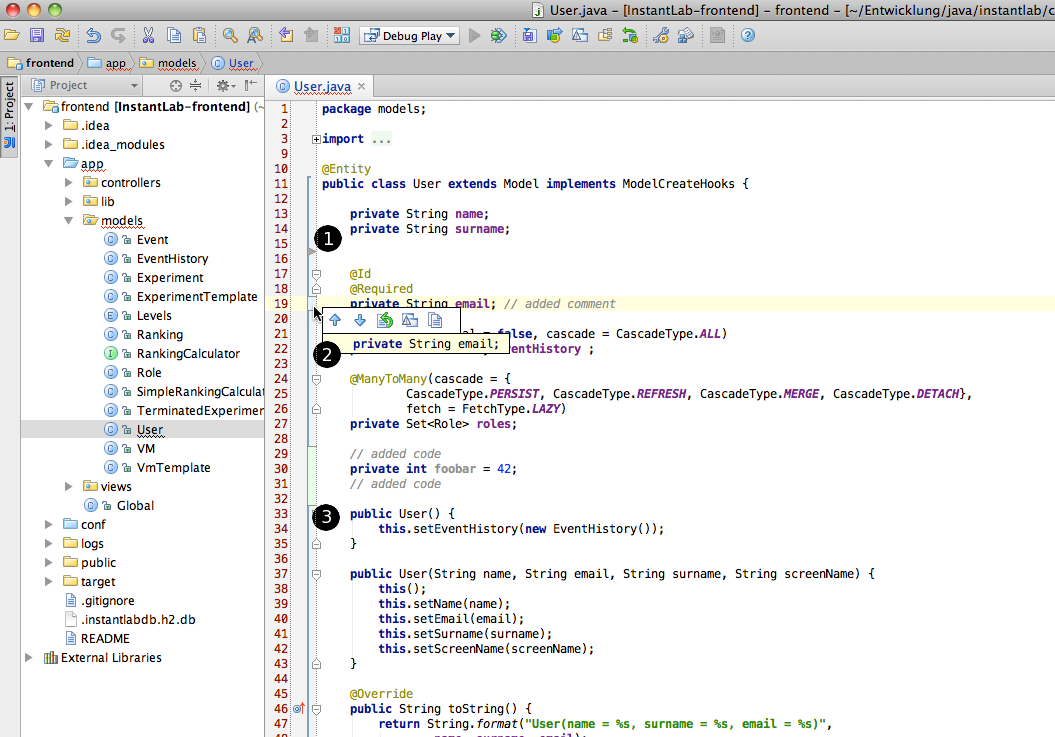
\includegraphics[width=0.9\textwidth]{images/idea-git.png}
	\caption{IntelliJ IDEA git integration}
	\label{fig:idea}
\end{figure}

In Figure ~\ref{fig:idea} you can see a screenshot of IntelliJ IDEA's code editor including the live diff.
At \circnum{1} there is a little gray triangle which marks deleted code.
You can see the deleted code by clicking on it.
Changed lines are marked via a blue strip on the editor's gutter (\circnum{2}).
By clicking that strip the original code is displayed.
Finally, as seen at \circnum{3}, added code is marked by a green strip.

\subsection{gitx}
\label{sec:gitx}

Bundled with git comes a graphic tool called \emph{gitk} with which you can review local changes
and the history of your git repository. There are several similar tools that offer additional features.
One of those tools is \emph{gitx} for MacOS and one of the additional features is the ability to partially apply and revert
changes, while usually IDEs such as IntelliJ IDEA only allow you to commit files as a whole.

\begin{figure}
	\centering
	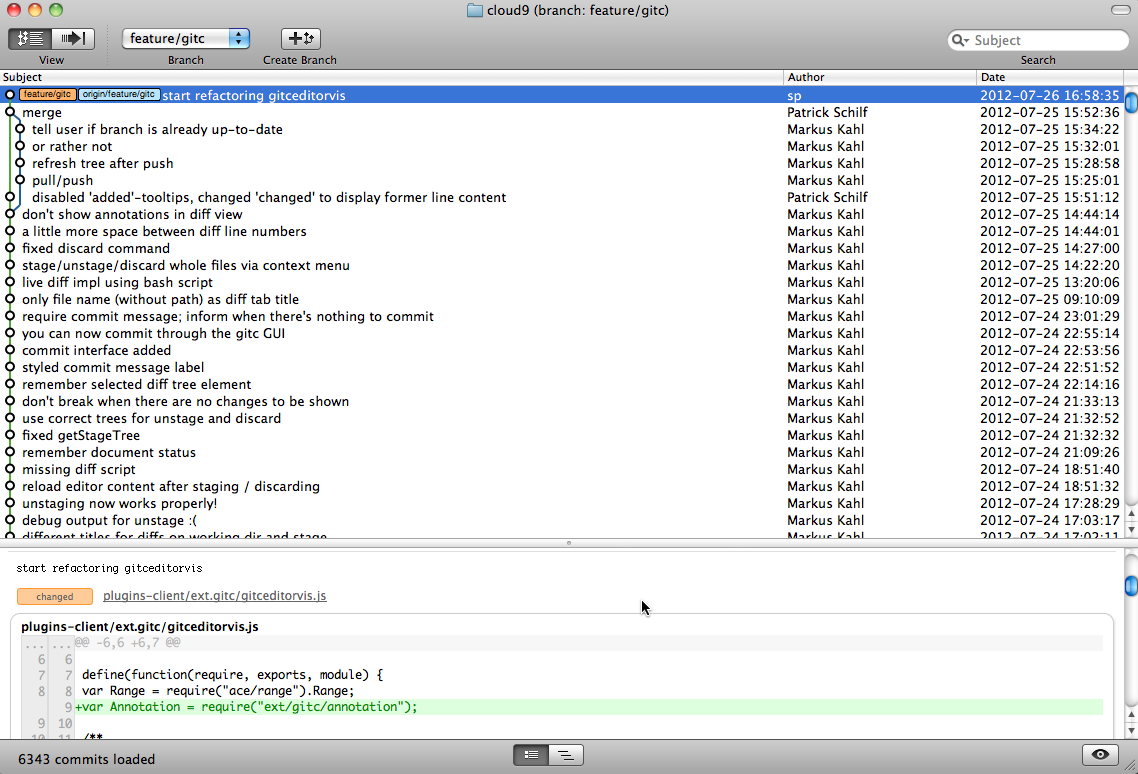
\includegraphics[width=0.9\textwidth]{images/gitx-history.png}
	\caption{gitx history view}
	\label{fig:gitx-history}
\end{figure}

Figure ~\ref{fig:gitx-history} shows gitx's history view where you can see the list of all commits.
Below the list of commits the diff for the selected commit is displayed.
Currently Cloud9 only provides a history of local changes independently from git. Another feature \emph{gitc} is supposed to add
is this git history view. Although it hasn't been implemented, yet.
\vspace{11 pt}

\begin{figure}
	\centering
	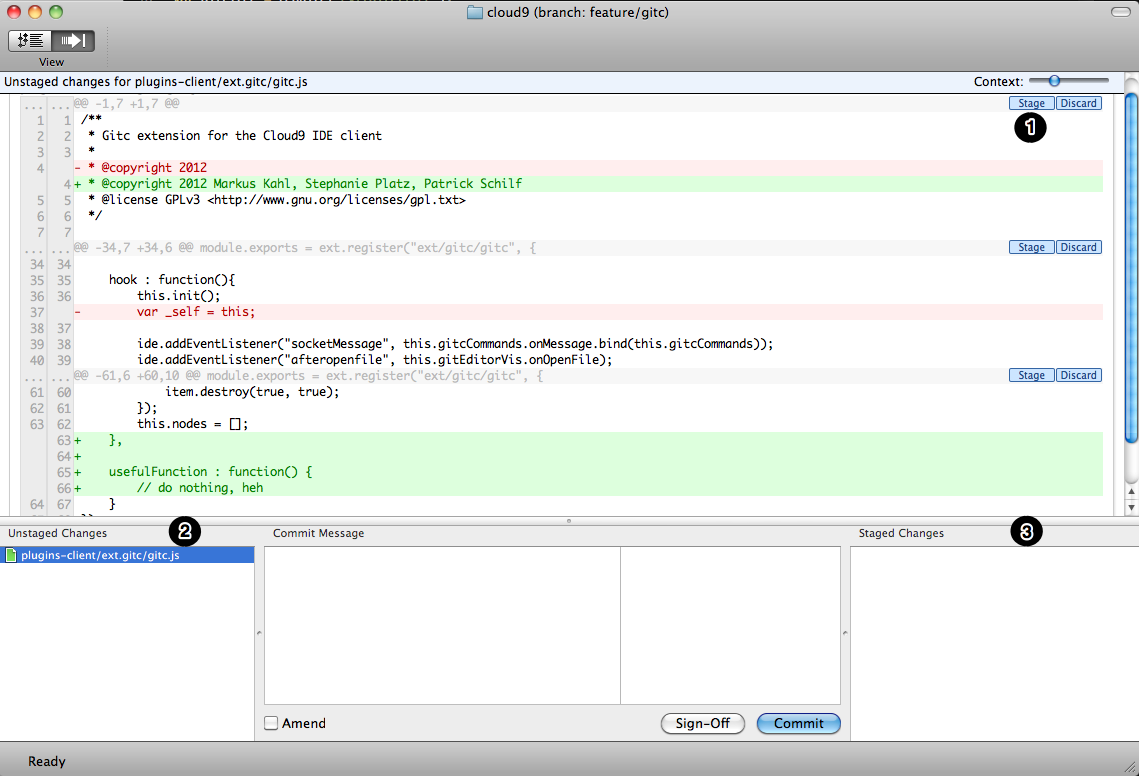
\includegraphics[width=0.9\textwidth]{images/gitx-commit.png}
	\caption{gitx commit view}
	\label{fig:gitx-commit}
\end{figure}

You can see gitx's commit view in figure ~\ref{fig:gitx-commit}. It shows the diff for local changes grouped into several so called hunks by git.
It's also possible to commit those separately by using the command line (\emph{git add --patch}), though gitx offers a more
convenient UI.
As you can see at \circnum{1} there are stage and discard buttons at every hunk.
Through this you can either add separate hunks to the next commit or revert them.
Staged changes will go from \circnum{2} to \circnum{3} and can be unstaged again separately as well. %markus
\section{gitc extension}
\label{sec:Extension}
In this section we describe how a cloud9 user can work with our extension and we show how the developing workflow is improved by it.
Further we compare our extension to other tools introduced in section~\needcite{related work}.
Finally we will explain how we intregrated our extension to cloud9 and how we implemented it.

\subsection{gitc User Interface}
\label{sec:gitc_ui}
\paragraph{The editor adjustments} of our extension will promt the cloud9 user immediately with visiual feedback of source code changes.
That means while typing within the editor makers will appear next to the left grutter line as can be seen in figure~\ref{fig:editor}.

The changes show the staged and unstaged changes of the git repository respectively.
We choose to display those both types of changes as colored markers whereas the already staged changes are more transparent.
In the upper screenshot of the cloud9 editor are only unstaged changes displayed.
The lower screenshot shows that the state of the git repository is changed.
Some of the changes are staged and at~\circnum{2} and~\circnum{3} are some (new) unstaged changes.
So in the line marked by~\circnum{2} there are both staged and unstaged changes visualized.
The colors green, blue and red are used to visualize added~\circnum{3}, changed~\circnum{2} and deleted~\circnum{1} lines respectively.

Furthermore the user will get tooltips hovering over one annotation.
In this way deleted lines or the old content of changed lines will be displayed to the user.
We do not provide buttons to stage, unstage or discard the changes because there is already an extension which allows developers to go back in history (see figure~\ref{fig:history}).
As for the staging and unstaging we want to have an overview over all current changes and thus rather use the diff view than search in single source code files for changes.

\begin{figure}
   \centering
   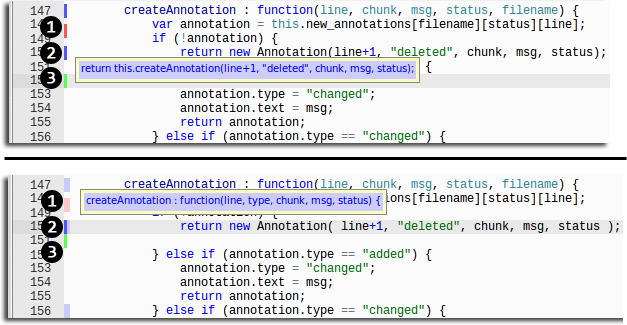
\includegraphics[width=0.9\textwidth]{images/extension_tooltip_comparison.png}
   \caption{Editor adjustments of our cloud9 extension gitc.}
   \label{fig:editor}
\end{figure}

\paragraph{Using our diff view} the cloud9 developer has now a view to explore \texttt{git diff} visually (see figure~\ref{fig:diff_view}).
By clicking on the pane button~\circnum{1} or simply using the keyboard shortcut \texttt{strg + g} / \texttt{cmd + g} the diff view will be opened.
The tree view at the left is filtered for changed files only.
The icon of an item of the tree will indicate the change state.
A green plus, a blue star and a red minus signify added, changed or deleted files respectively.
At the top~\circnum{2} the unstaged changes and at the bottom~\circnum{3} the staged changes are listed.

Double clicking on a file will open its changes in the editor.
Deleted or added lines will be marked with a red or green backgound and line numbers are displayed in two columns.
The left column shows the line number in the old file and the right column shows the line number in the new file.
For each single hunk there is a small menu with according options~\circnum{4}.
This is either to \emph{discard} or \emph{stage} unstaged hunks or \emph{unstage} staged hunks.
As soon as all belonging together hunks are staged developers can type summarizing message and click the commit button~\circnum{5}.
To pull and push from the git repository we provide context menu entries~\circnum{6}.

\begin{figure}
   \centering
   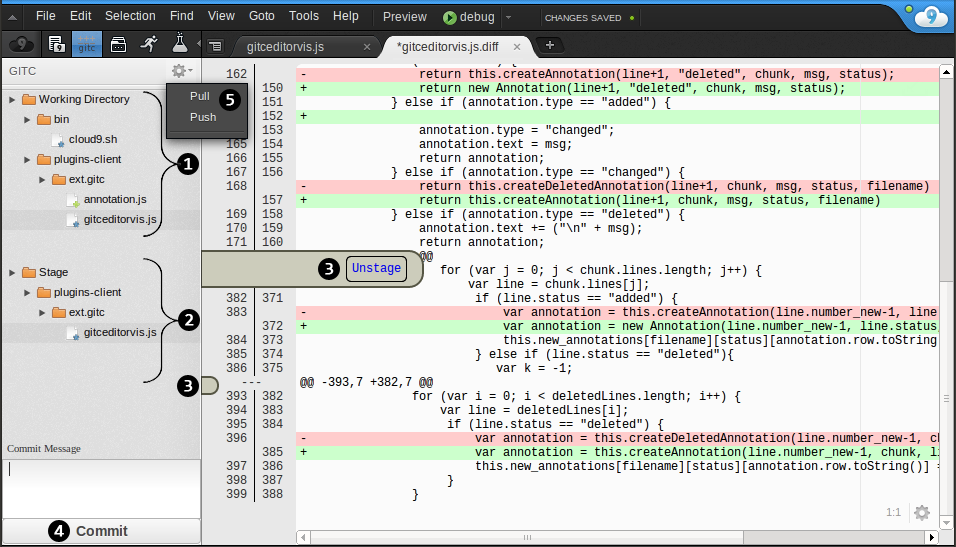
\includegraphics[width=0.9\textwidth]{images/extension_unstage.png}
   \caption{The diff view of our cloud9 extension gitc.}
   \label{fig:diff_view}
\end{figure}

\subsection{Workflow Improvement}
With our extension developers get realtime feedback of \texttt{git diff} of the current opened file while editing it.
This is visualized in a similiar way as stated in section~\ref{subsec:IntelliJ_IDEA}.
But we decided to not put buttons in our tooltip but to show the older content.
On the one hand because of the history extension (figure~\ref{fig:history}) enabling to discard changes.
On the other hand we figured out that mostly changes are scattered within one file or often over several files and thus buttons to stage and unstage hunks might not be that useful in a editor.
As a result there is no longer a need to switch back and forth from editor to console as we had before (see section~\needcite{our workflow}).

Once a developer decides to commit his changes he can switch via click or keyboard shortcut to our diff view.
Here it is possible to rapidly execute a bunch of git commands by simply clicking on certain buttons.
This replaces the missing interactive console to stage seperate code hunks and to only view a snippet of a diff.
Further we colorized changed lines as proposed in section~\ref{subsec:ext_git_integration} and~\ref{subsec:gitx}.

\todo[anything forgotten???]

\subsection{Implementation}
Cloud9 has a plug-in architecture.
Therefore we implemented our gitc extension as a plug-in.
Whereas there are examples how to implement a cloud9 plug-in we had difficulties finding further documentation for cloud9 internals as well as for cloud9 third party software.
Thus we struggeled first finding out how to send git commands and later with the integration into the apf\footnote{\url{ace.ajax.org/api/}} and Ace editor.

In the following subsections we will describe how we implemented our extension.
First we will have a closer look at how we intregrated our extension to cloud9 and how we execute git commands.
Then we will explain how we implemented the adjustments in the cloud9 editor and the new diff view.

\subsubsection{Sending git commands}
%client-side, server-side hook
%sending commands (channel)
%reacting to commands
%git parser
%following two are as well client-side

To send git commands our plug-in has to register on client-side and server-side to the cloud9 ide.
Thus we implemented a client-side interface that can send a command to the server-side, catch the resulted output and then call a callback, if given, with this output.
As for that we have to give ids to those command to assign the output to the right callback.
To then interpret that output we implemented a git diff parser as well. 

On the server-side we filter all out gitc commands and spawn the rightful command as a shell process.
To regocnize our commands we use an own channel for them.
This additionally prevents other extensions reacting to our commands.
If then output messages will be send via our channel we collect them and send them back to the client.

Because we can only execute git commands on the server-side (which is caused by the Cloud9 architecture) there might be performance issues when the connection is not good enough.
There are possible situations when it is not necessary to send a git command so we should improve our code at according places and save those commands.
Further we wish to execute \texttt{git commit} when being offline.
Both issues might be solved by using git.js (see~\ref{sec:offline-git-support}).

\subsubsection{Editor Adjustments}
%ask for git diffs when creating document
%creating and storing annotations, unsaved changes
%using ace api: markers
%registered events: document creation, tab switch, document change

Once a document is opened or becomes active for the first time in the editor, its current workspace version is checked against the repository version. 
For that purpose gitc registeres with the \texttt{documentCreate} and \texttt{tabSwitch} events emitted by the cloud9 ide. 
Sending the command \texttt{git diff [--cached] -U0} to the client side gitc interface returns the unstaged [staged] differences between the two file versions, split into the various chunks. 
Staged and unstaged changes for each document file are transformed into objects that we refer to as \texttt{annotations} and maintained in an array. Annotations are constantly updated as long as the user edits the document. 
Once saved, the document is checked against the repository version again and the annotations array is refilled. 
Ace provides \texttt{documentChange} and cloud9 ide \texttt{saveFile} events in order to keep track of change and save operations introduced to the document file. 
In order to highlight code changes according to annotations, Ace stores various states related to a document in an \texttt{EditSession}, which provides a function \texttt{addMarker}. 
A marker is a highlighted range of text or text background over one or more lines in the editing window. 
In our implementation we make use of markers in order to produce the narrow bars at the left border of the window as already described in \ref{sec:gitc_ui}. 
Markers are created and updated every time a document is opened, saved or edited. 
Subscribing to the Ace event \texttt{mouseMove} enables hovering elements in the code window, which we use to create our tooltips that relate to code changes as in figure~\ref{fig:editor}.

\subsubsection{Diff View}

Pressing Cmd + G opens the gitc panel which shows the current changes as shown in figure ~\ref{fig:diff_view}.
Cloud9 uses APF\footnote{Ajax.org Application Platform - \url{http://ui.ajax.org/#home}} as the basis for the whole application.
Defining the gitc panel involves putting together an xml markup (AML) file describing the UI.
There is documentation\footnote{\url{http://ui.ajax.org/#docs}} which helps you build your markup to get the desired UI.
However, there is a lack of examples showing how to actuallly use the UI elements. Things such as processing a click of button
or how to fill and change a tree.
In the end we still managed to implement everything we wanted through experimentation and looking through the code of the core
and other plugins.

For the display of the actual diff inside the editor we had to resort to overriding the editor's update function to be able to
render our own gutter with custom line numbers as required by the diff.
 %stephi: description, new workflow, ansonsten jeder seins
%\include{chapters/evaluation} ???
\section{Future Work}
\label{sec:Future_Work}

While we are quite satisfied with the features we managed to implement in the given time,
there is more to be done to make the git integration perfect.
Most importantly the \emph{history view}, but also:
\begin{itemize}
	\item switching branches
	\item checking out specific tags/commits
\end{itemize}
An optional but potentially very useful feature would be \emph{offline} git support.

\subsection{History View}
\label{sec:history-view}

For completion gitc should also feature the history view shown in figure ~\ref{fig:gitx-history}.
This would not necessarily have to look just as in gitx.

\subsection{Branches and checkout out specific tags and commits}
\label{sec:branches}

Currently \emph{gitc} does not support branches. Creating branches as well as checking out branches,
commits etc. still requires the use of the Cloud9 console. It would be desirable to be able to do all
this over the \emph{gitc} view.

\subsection{Offline git support}
\label{sec:offline-git-support}

There is one major restriction while working with git through Cloud9. It does not work offline since everything goes through the Cloud9 server-side component.
Usually this would not be a problem, however it is one of the key points of git that you can work with it (committing etc.)
while offline.
It would be very useful if you could still do at least some things while offline.
Perhaps one could realize that through Dan Lucraft's git implementation git.js\footnote{\url{https://github.com/danlucraft/git.js}} in pure Javascript which we could possibly run on the client side to do local commits for example.

\subsection{Production}
We are in contact with the Cloud9 team and plan on getting our plugin production ready so that it can be integrated into the main Cloud9 IDE. %markus
\section{Conclusion}
\label{sec:Conclusion}

In this paper, we presented gitc, a Cloud9 extension that allows for a better programming experience when working with git. 
Based on our sample implementation of \textit{Tetris}, we evaluated possible Cloud9 features that would considerably improve the IDE and could be reasonably implemented in the time range of one semester.
Gitc provides experienced git users with the functionality and usability they already know from desktop tools. 
By tracking and displaying code changes they receive immediate feedback on their actions. 
Creating this "immediate connection" was one of our initial goals of this seminar. 
Gitc also makes git newcomers learn the git process in a much quicker and more comfortable way. Buttons that are placed right where code changes happen lead the user through the git stage-commit-push workflow and give them an intuitive understanding of what a chunk is.

Technically, although we managed to achieve most of our goals, there is still room for potential improvements. 
Most of all performance of realtime updates of code changes needs to be tested in a real world environment. 
Since we could only run and develop in a local environment, optimizations may become necessary. 
We also think of additional features, that we think would yet further improve the experience of our tools. 
Section ~\ref{sec:future_work} gives an overview of potential features.

Our implemented features address the issues with the current Cloud9 version. 
We've been contacted by the Cloud9 team and work together on getting \emph{gitc} into the main Cloud9 IDE\footnote{\url{http://c9.io}}. %patrick

\bibliographystyle{plain}
\bibliography{cloud9-Refs}

\end{document}

%\begin{figure}
%	\centering
%	\includegraphics[width=\textwidth]{images/picture.png}
%	\caption{A nice Caption}
%	\label{fig:Caption}
%\end{figure}